\documentclass{article}

%%%%%%% PACKAGES %%%%%%%%
\usepackage[utf8]{inputenc}
\usepackage[margin=2cm]{geometry}
\usepackage{blindtext}
\usepackage{setspace}
\usepackage{graphicx}
\usepackage{notoccite} %citation number ordering
\usepackage{lscape} %landscape table
\usepackage{caption} %add a newline in the table caption
\usepackage{float}
\usepackage{color}
\usepackage[dvipsnames]{xcolor}
\definecolor{ultramarine}{HTML}{2f3973}
\definecolor{hexablack}{HTML}{000000}
\usepackage[colorlinks = true,
linkcolor = hexablack,
urlcolor  = ultramarine,
citecolor = ultramarine,
anchorcolor = hexablack]{hyperref}

\title{\huge{\textbf{Gesture Based UI Development}} \\
\LARGE{Research Paper}}
\author{John Shields}
\date{February 2021}

\begin{document}
\pagenumbering{roman} % Start roman numbering
\clearpage\maketitle
\thispagestyle{empty}
\begin{center}
    \begin{figure}[h]
        \centering
        
\includegraphics[width=15cm]{pics/logo-gmit.png}
        %\caption{Your caption here}
        \label{fig:logo}
    \end{figure}
    \large{	BSc (Hons) in Software Development \\
    Lecturer: Damien Costello}
\end{center}
\newpage
\setcounter{page}{1}
\tableofcontents
\listoffigures

\newpage
\pagenumbering{arabic} % Start roman numbering

%%% CONTENT START HERE %%%%
\section{Description}
This Research Paper is based on Gesture Based User Interface Experience that focuses on Accessibility, Evolution, and Challenges. The purpose of this paper is to research the User Interface as it moves from purely physical (mouse, keyboard, touch screen) to include intuitive interaction through gestures.

\section{Introduction}
Gesture Based User Interface Experience can vary in many ways. Computers are all around us. It can be said that almost every household has at least one computer, where it be a PC or a Laptop, there is sure to be one in most homes today. Obviously, computers are not the only devices in homes. Nowadays, Phones are extremely popular and heavily used. They might even be used more than computers. Having said that, a phone is basically a computer that you can fit in your pocket. Gesture Based UI is heavily used in these devices. This can be as simple as sliding your hand to the left and right to go back and forth between pages for a computer. Gestured Based UI only came into play with phones when the touch screen was introduced. Computer too can have touch screens, but it is optional. Most personal phones likely have touch screens. Today's phones rely on the touch screen. They only have a few physical buttons. These are mainly for locking/unlocking phones and for adjusting the volume level. Gesture Based UI is not just for computers and phones. It is also for something as simple as a watch or a car radio, making them smarter. Gestured Based UI makes every device smarter.

\section{User Experience Evolution}
\subsection{Early Days of User Experience}
User Experience is constantly Evolving. The first general-purpose computer was the monolithic ENIAC machine. The machine's construction began on the 13th of May, 1943, and was finished on the 2nd of October, 1955. The User Experience on the ENIAC was a bit of a headache and relied on many experts to work the machine. ENIAC was designed to be capable of being reprogrammed to solve a large number of numerical problems. The machine's programming consisted of setting switches and connecting wires according to specific instructions, which were first worked out on paper, which took weeks. This machine also used a punch-card reader as an input and output device. This is obviously not very user-friendly, but for the time, it was extraordinary. Comparing this machine to any computer or smart device today shows how much these technologies have evolved.
\cite{ref1}

\begin{figure}[h!]
    \caption{ENIAC Machine}
    \label{image:ENIAC}
    \centering
    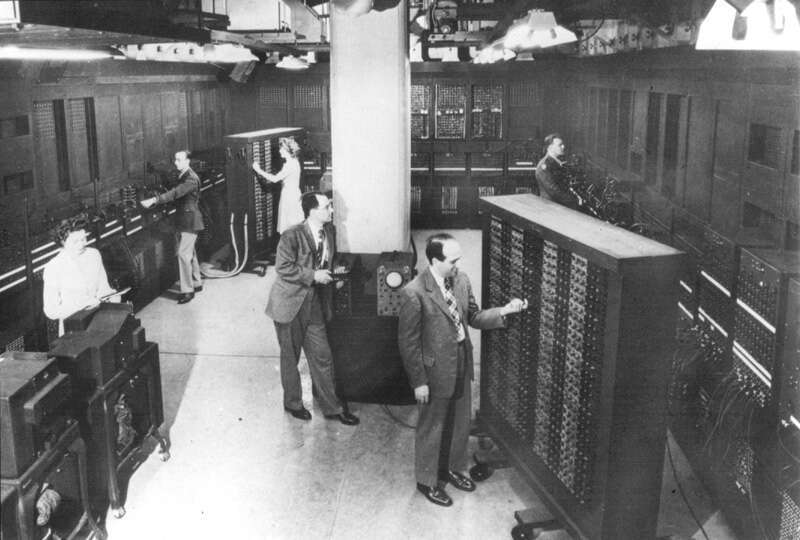
\includegraphics[width=0.6\textwidth]{pics/eniac.jpg}
\end{figure}
\newpage
\subsection{The Computer Keyboard}
One of the key parts of a computer that is still highly used today is the keyboard. Typewriters inspire keyboards. The typewriter has been around since the late 1800s and is an antique that is still used today. The QWERTY keyboard layout, which came from the Sholes and Glidden typewriter, also came from this time. QWERTY's design has the keys to be spread out to avoid jamming those old typewriters. The QWERTY layout has stood the test of time in the English speaking world. The Binac computer (1948) used an electromechanically controlled typewriter to input data directly onto magnetic tape and print results. This was the first integration of a keyboard like system for a computer and began the computer keyboard's origins. Since this origins, the keyboard is used in most electronic devices that require typing. 
\cite{ref3}

\begin{figure}[h!]
    \caption{The Binac Computer}
    \label{image:BINAC}
    \centering
    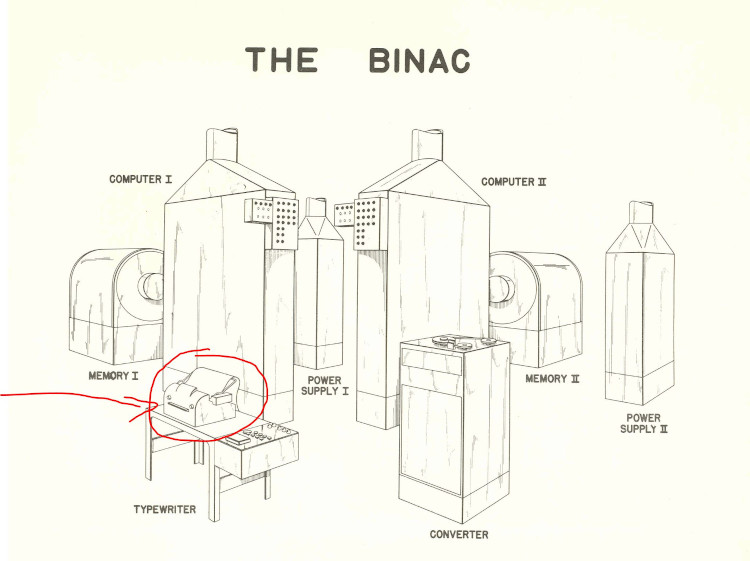
\includegraphics[width=0.45\textwidth]{pics/binac.jpg}
\end{figure}

\subsection{The Computer Screen}
What is a UI without a screen? A screen is so essential now and is probably the most important part of a computer. The ZUSE 3 (Z3) Computer (1941) was the first working programmable and fully automatic digital computer.  The Z3 was constructed with hundreds of relays, second-hand sheet metal, and mechanical pins. The Z3 had an output display that showed results on a light stripe, including the location of decimal commas. At the same time, computers from this time provided hard-copy printouts. Computers like the Z3 were dominated by a digital display that consisted of rows of blinking lights that flashed when the computer processed particular instructions or accessing memory locations. 
\cite{ref4} \cite{ref5}

\begin{figure}[H]
    \caption{The ZUSE 3 Computer}
    \label{image:ZUSE3}
    \centering
    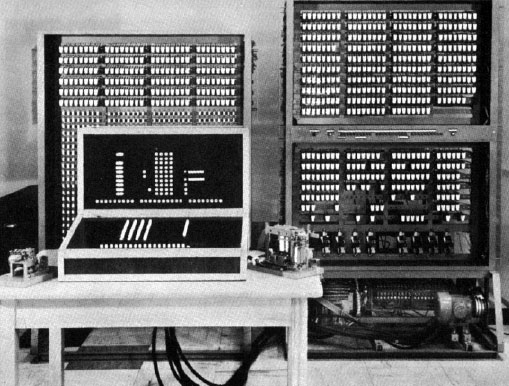
\includegraphics[width=0.5\textwidth]{pics/z3.jpg}
\end{figure}

Since the Z3, computers such as the SWAC Console and the Ferranti Mark 1 Star (1951) used CRT Display (Cathode-ray tube) to show CRT-based memory contents. In the 1960s, CRT was used as virtual paper in a virtual teletype on computers such as the Uniscope 300 (1964) and the ADM-3 (1975). These display terminals became very prominent for the UI in computers right into the mid-1970s. At the time, these computers were quite expensive, so they were not hugely accessible. In the mid-1970s, CCTV was used to create cheaper computers such as the Apple I (1976) and the SOL-20 (1976). These were the first computers that have factory video outputs. As a result, these computers became more accessible than their predecessors. With the Television (TV) becoming more and more popular, computers started to use the TV's technology. Companies like Apple, Commodore, and Radio shack used this technology to their advantage to create a better User Experience.

In the 1980s, computer screens became revolutionary with the use of CGA (Color Graphics Adapter) and EGA (Enhanced Graphics Adapter) that were both introduced by IBM. These brought colour and higher resolution to computer screens. Followed by these displays, the Macintosh Monitors came, and they used bitmapped graphics. The Mac II's (1978) video standard was quite similar to the VGA (Video Graphics Array). Mac monitors continued to evolve and were always known for their sharpness and accurate color representation.

Also, in the 1980s, LDC (Liquid Crystal Display) screens that originated from the 1960s became widely used on calculators and watches with monochrome displays—from the 1980s and on through the 1990s, LCD drastically improved. At this time, LCD created a market boom for laptops. LDC is continued to be supported and used today in electronic devices such as PCs, laptops, TVs, smartphones, smartwatches, cameras, Etc.
\cite{ref5}

\begin{figure}[!h]
    \caption{Modern Screens}
    \label{image:MODERNSCREENS}
    \centering
    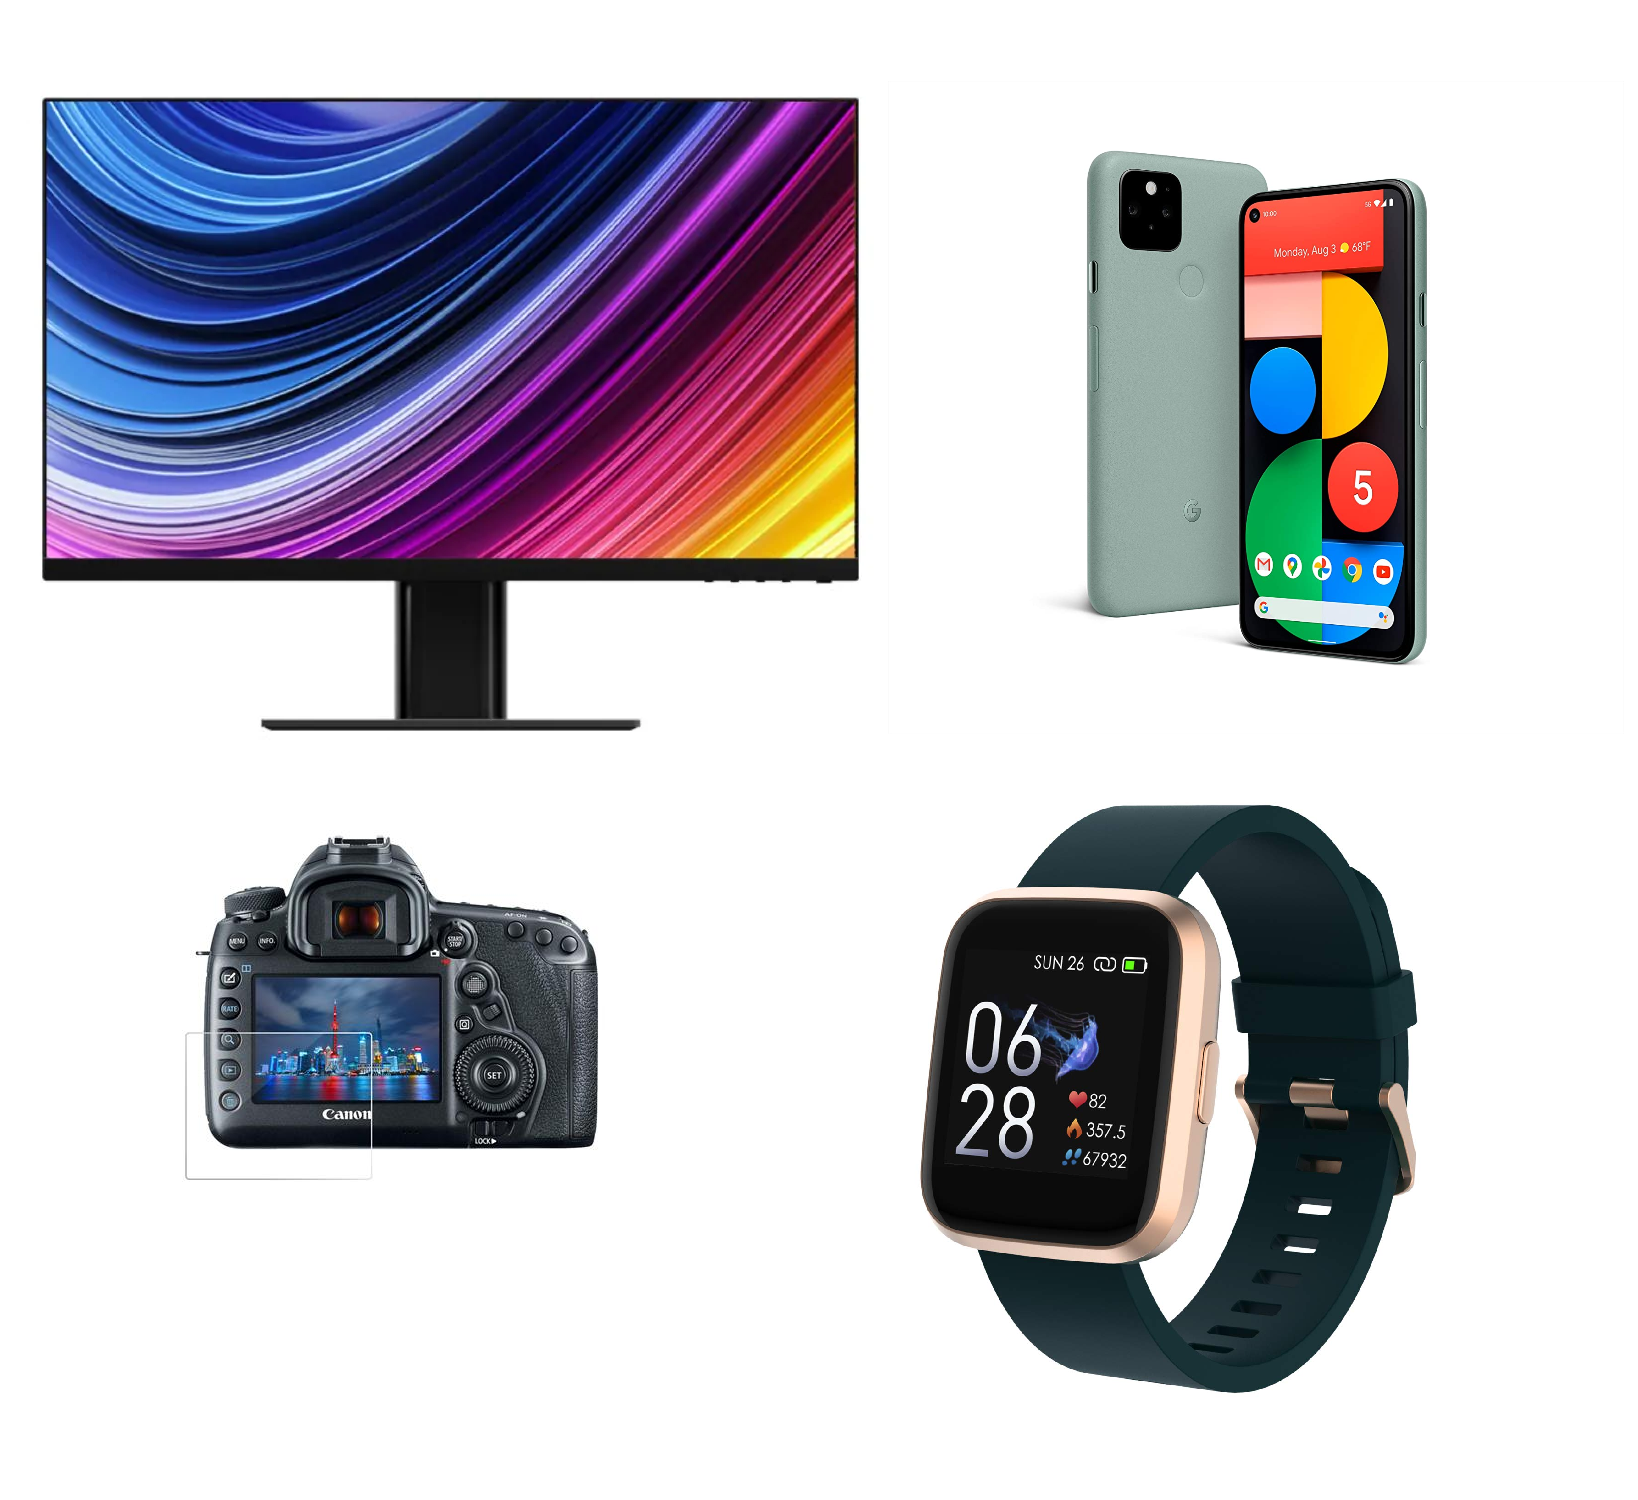
\includegraphics[width=0.5\textwidth]{pics/modern_screens.png}
\end{figure}

\subsection{The Computer Mouse}
The Mouse is another essential part of a computer. Before the use of the mouse, data was entered by typing commands with the keyboard, as discussed earlier. The common mice that are used today are made out of plastic. The first computer mouse was designed as a wooden box with two metal wheels that make contact with the surface and only one key. Douglas Engelbart invented this mouse in 1964. This mouse was pretty limited in what it could do. It was only eight years later that Bill English created the Ball Mouse. The ball replaced the two metal wheels that Engelbart's mouse, which made it possible for this mouse to move in every direction. The Alto (1973) had a special input interface made by SRI. Alto's mouse had three buttons and enabled the first bitmapped and overlapping windows display. As a result, Alto's became very popular with its users. D. Venolia of Apple developed the first scroll-wheel in the late 1980s. It was not until the 1990s that mice started to resemble present-day mice. In 1999 Microsoft created a mouse known as the Intellimouse with an Optic LED design. This mouse paved the way for a new generation of optical mice.
\cite{ref6} \cite{ref7}

\begin{figure}[!ht]
    \caption{Computer Mice Throughout the Years}
    \label{image:mice}
    \centering
    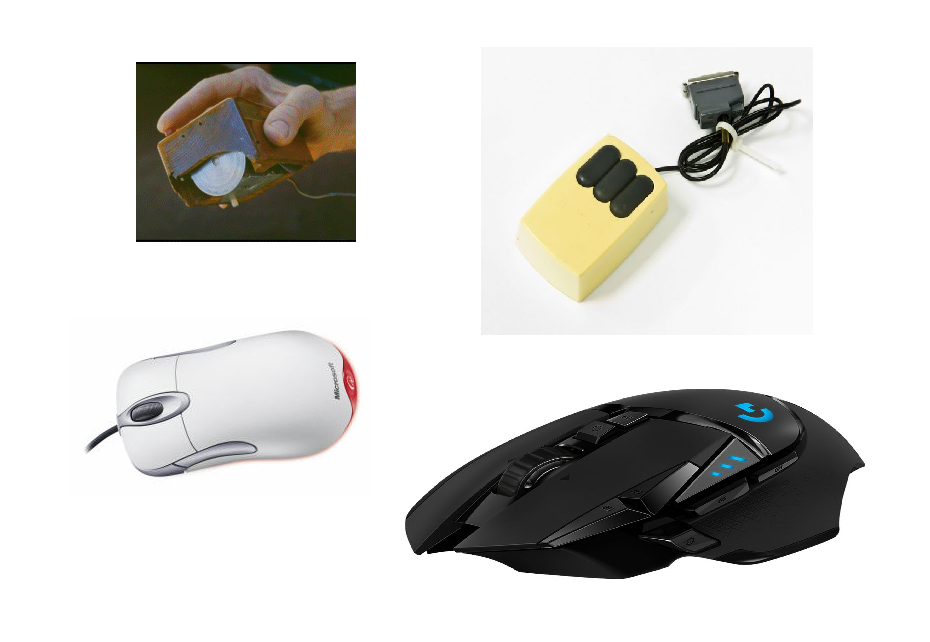
\includegraphics[width=0.5\textwidth]{pics/mice.png}
\end{figure}

\newpage
\subsection{The Touch Screen}

\subsection{Voice Control}

\subsection{Virtual and Augmented Spaces}

\subsection{Gesture Recognition}

\section{Gestures as a Communication Tool}

\section{Challenges for the Design of Applications}

\section{Challenges for Implementation}

\section{Conclusions}

 \newpage
 \begin{thebibliography}{00}
    
\bibitem{ref1} History of Computers
\newline
URL: \url{https://homepage.cs.uri.edu/faculty/wolfe/book/Readings/Reading03.htm}

\bibitem{ref2} SUZANNE DEFFREE - EDN - Construction begins on ENIAC
\newline
URL: \url{https://www.edn.com/construction-begins-on-eniac-may-31-1943/}

\bibitem{ref3} Mary Bellis - The History of the Computer Keyboard
\newline
URL: \url{https://www.thoughtco.com/history-of-the-computer-keyboard-1991402}

\bibitem{ref4} History Computer Konrad Zuse
\newline
URL: \url{https://history-computer.com/konrad-zuse/}

\bibitem{ref5} Benji Edwards - PC world - A brief history of computer displays
\newline
URL: \url{https://www.pcworld.idg.com.au/slideshow/366677/brief-history-computer-displays/}

\bibitem{ref6} Jessica Z - Sutori - HISTORY OF COMPUTER MOUSE
\newline
URL: \url{https://www.sutori.com/story/history-of-computer-mouse--2yUFPn6vNQBstaaz2x4FTdsy}

\bibitem{ref7} Bill Buxton - Some Milestones in Computer Input Devices
\newline
URL: \url{https://www.billbuxton.com/inputTimeline.html}

\end{thebibliography}

%%% CONTENT HERE END %%%%
\end{document}
\newpage
\setstretch{1}  %reduce bibliography line spacing
\printbibliography
\end{document}